\section{Evaluation}
\label{sec:evaluation}
We evaluated our hardware design for a \name{} running at 3 GHz, and compared its performance to an unmodified RISC-V core with a standard NIC (IceNIC), which we will call ``Traditional.'' 

\begin{figure*}
  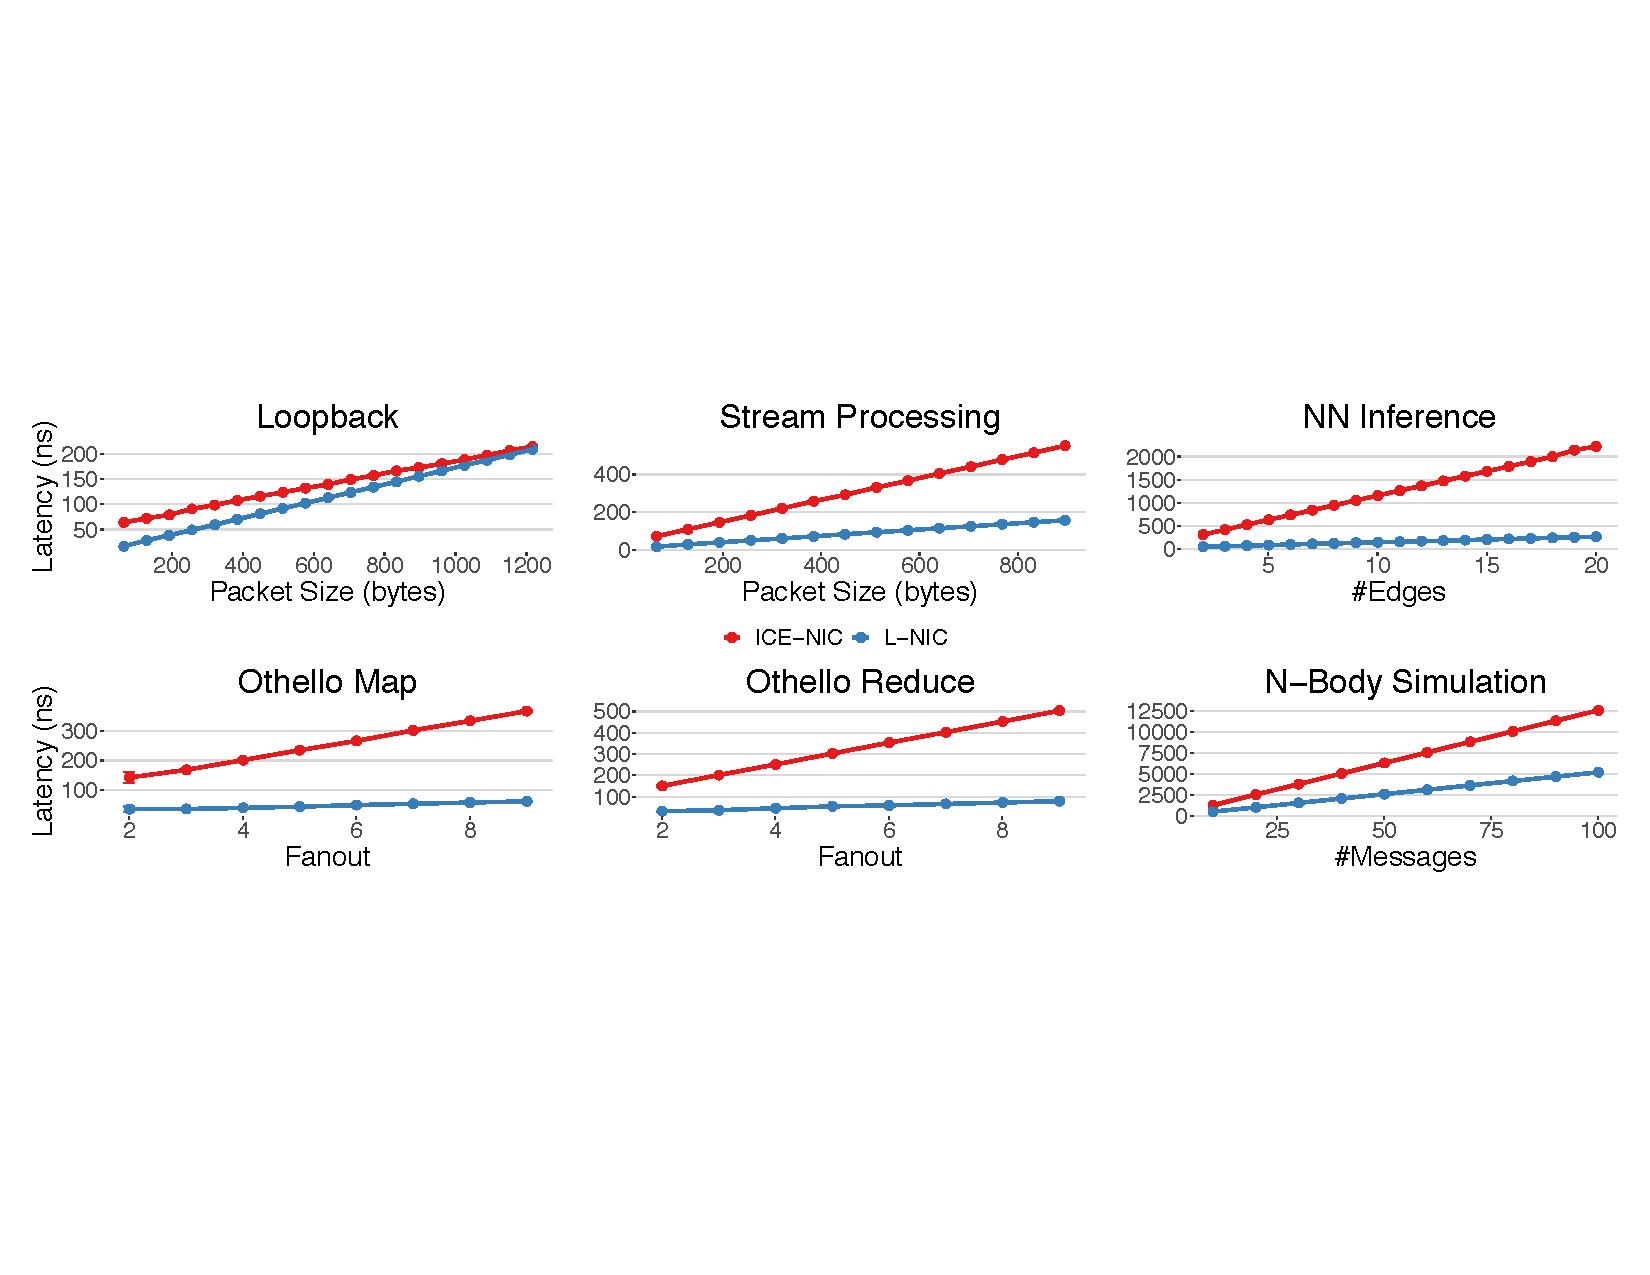
\includegraphics[width=\linewidth]{./figures/latency}
  \caption{Nanoservice application latency comparisons for \name{} vs a traditional RISC-V core with IceNIC.}
  \label{fig:latency}
\end{figure*}

\subsection{Microbenchmarks}
We wrote and ran microbenchmarks for three main aspects of our \name{} design. 

\paragraph{Timing Analysis.} We wanted to know if a \name{} runs more slowly than the Traditional design. We synthesized both designs to run on a modern FPGA (Xilinx Ultrascale+). In both cases the critical timing path was the L2 cache, and hence our \name{} prototype runs at the same speed as the unmodified RISC-V system.

\paragraph{Basic Latency/Throughput Performance Analysis.} 
Figure~\ref{fig:latency}a compares the loopback latency, as a function of packet length, for both designs. For short packets, \name{} latency is 4$\times$ shorter than for the Traditional design. This should come as no surprise: The \name{} transmit path is only 11 clock cycles ($<4$ns at 3GHz) for a single word message, measured from when an application writes the word into the register until it is placed on the network (not including the MAC processing). And the \name{} receive RX path is only 6 cycles (not including the MAC processing). For longer packets the loopback for the two designs eventually converges as the latency becomes dominated by store-and-forward delays. 

\Cref{tab:throughput} compares the TX and RX throughput for 64B packets for both designs; the \name{} runs at 6--8$\times$ higher throughput than the traditional design, mostly because of the huge reductions in per-packet overheads in the \name{}.
A \name{} application does not need to take time to instruct a DMA engine to send/receive packets, it simply reads and writes the NIC queues directly. We could expect the IceNIC throughput to increase slightly if it supported descriptor rings, which means the application doesn't need to program the DMA for every packet. However, this would also increase latency, because of batching.

% \steve{My main concern with using IceNIC as a baseline comparison is that it does not support TX/RX descriptor rings, which means that the application must send packet descriptors one at a time to the NIC DMA engine for TX and the NIC DMA engine only fills up one packet buffer at a time for RX. I don't think this matters too much for latency of a single packet, but throughput will be affected. For example, the TX/RX throughput for 64B packets would be higher for IceNIC if it supported this feature. Additionally, the IceNIC applications might be written differently. For example, rather then using the same static buffer for every packet, they might use N packet buffers and process them in batches. So it's tough to say what the performance impact would be on the evaluated applications. I tried measuring the performance gain resulting from support for descriptor rings by writing a DPDK (actually MoonGen) application that sends/receives 1 pkt at a time vs batches of packets. The results were unfortunately inconclusive because DPDK is able to saturate the 10G link when sending batches of 64B pkts. Sending one 64B pkt at a time resulting in about 2Gb/s throughput. But this isn't really the right experiment to be running. The best thing to do if we had more time would be actually implement our nanoservice apps using DPDK and measure the latency using NetFPGA. If we did this, we would be able to compare the performance directly to our \name{} and IceNIC. Perhaps it's worth doing this for the camera ready?}

\begin{table}
\begin{center}
\begin{tabular}{c|c|c}
                          & \textbf{RX (Gb/s)} & \textbf{TX (Gb/s)} \\ \toprule
\textbf{The \name{}}     & 116                & 186                \\
\textbf{RISC-V w/ IceNIC} & 14                 & 28                 \\
\end{tabular}
\vspace{5pt}
\caption{Throughput for 64B packets. The \name{} prototype versus traditional RISC-V core with IceNIC.}
\label{tab:throughput}
\end{center}
\end{table}

%\begin{figure}
%  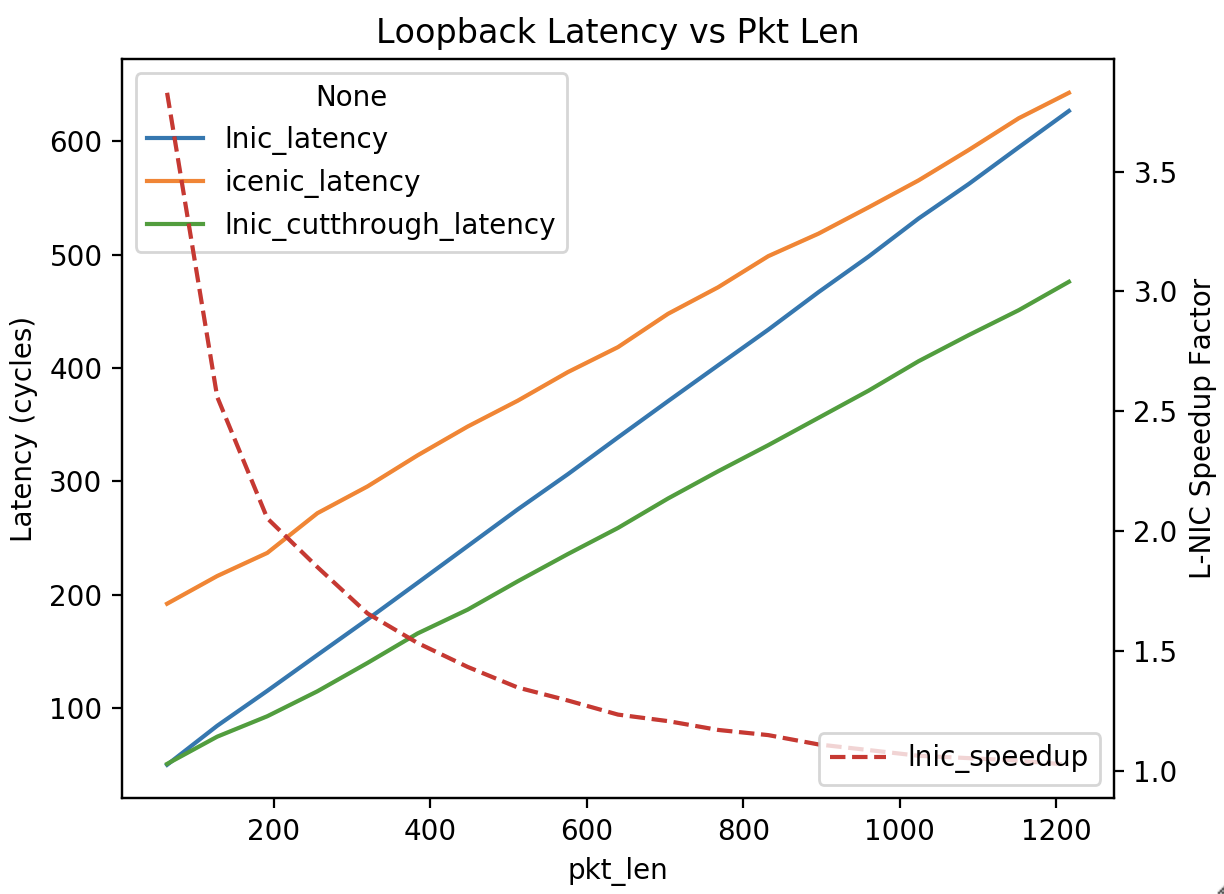
\includegraphics[width=\linewidth]{./figures/loopback-latency}
%  \caption{\name{} vs Traditional net-core-net loopback latency for various packet sizes.}
%  \label{fig:loopback-latency}
%\end{figure}

\paragraph{Thread Scheduler Latency.} We define the latency of the thread scheduler to be the time from when an interrupt fires to the time when the first instruction of the newly selected thread is executed.
We measured it to be \SI{60}{ns} (180 clock cycles) on the \name{} with almost no variation. This is at least two orders of magnitude faster than the best-known software schedulers~\cite{shenango}; and better still, has almost no variance, reducing the tail latency.

\subsection{Bare-Metal Application Benchmarks}
\label{ssec:bare-metal-evals}
We implemented and evaluated four nanoservice applications, and compared their performance on our \name{} prototype with the Traditional design. 

\paragraph{NFV-like Streaming Application.} This application emulates a very simple streaming NFV application. It treats an arriving message as a list of 8 byte unsigned integers, increments each integer, and then returns the resulting message back to the sender.
Latency is measured from the time when the first byte of the request enters the NIC to when the last byte of the response leaves the NIC.
Figure~\ref{fig:latency}b shows that the \name{} has 3.5--4$\times$ lower latency for all packet lengths. Note that the \name{} runs almost as fast as it did for the basic loopback, whereas the Traditional design runs much slower because the CPU is forced to touch every data byte in the packet. Every byte of the packet must be copied from memory into registers, then copied back to memory and then wait for the DMA engine to send it to the NIC. The \name{} eliminates all this overhead.


% Note that this type of application meets the criteria outlined in Section XXX to be considered a nanoservice application.
% Each message is processed independently, so it is highly parallelizable.
% Since NFV applications typically need to process messages as fast as possible, it is reasonable to expect that they will want to process each message within a microsecond.
% The simple example of an NFV style streaming application evaluated here is stateless between packets and hence the working set only needs to be large enough for the local computation, which in this case, is small enough to reside in the register file and never touches memory at all.
% Other NFV applications such as firewalls or intrusion detection systems would have a larger working set, especially if they need to match against a large list of rules.
% As long as this working set is cache resident, the application can be considered a nanoservice.

%\begin{figure}
%  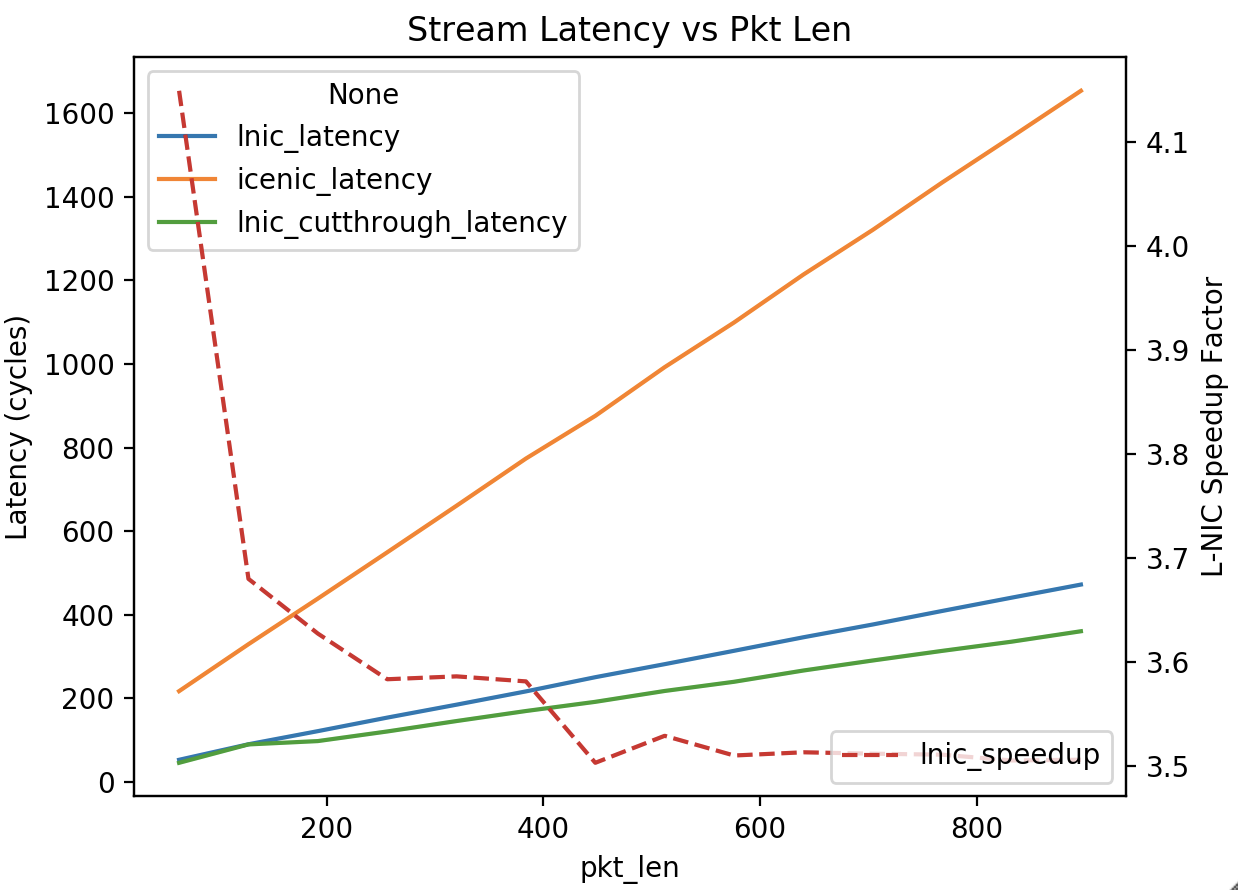
\includegraphics[width=\linewidth]{./figures/stream-latency}
%  \caption{\name{} vs Traditional NFV-style streaming application latency for various packet sizes.}
%  \label{fig:stream-latency}
%\end{figure}

\paragraph{Neural Network Inference.} The \name{} core can minimize the latency required for inference by exploiting the maximum amount of model parallelism. In inference, if each node runs a small number of multiply-accumulate operations, it can be turned into a nanoservice, particularly if the weights and data use reduced precision integers, as is typical in today's inference engines~\cite{tpu}.

We benchmarked inference for one node in a neural network by implementing a multiply-accumulate operation. The node receives $N$ weight messages and $N$ data messages, one for each incoming edge, then multiplies the corresponding data and weights and accumulates the result.
When all messages have been processed it sends a response message with the final result.
The latency is measured from the first byte of the first incoming message to the last byte of the response.
Figure~\ref{fig:latency}c shows that the \name{} implementation has an order of magnitude lower latency than the Traditional design. 
This is because (1) packet data does not need to be copied from memory to registers before using the ALU, and (2) the \name{} has a much higher RX throughput for small packets (as shown in Table~\ref{tab:throughput}).

%\begin{figure}
%  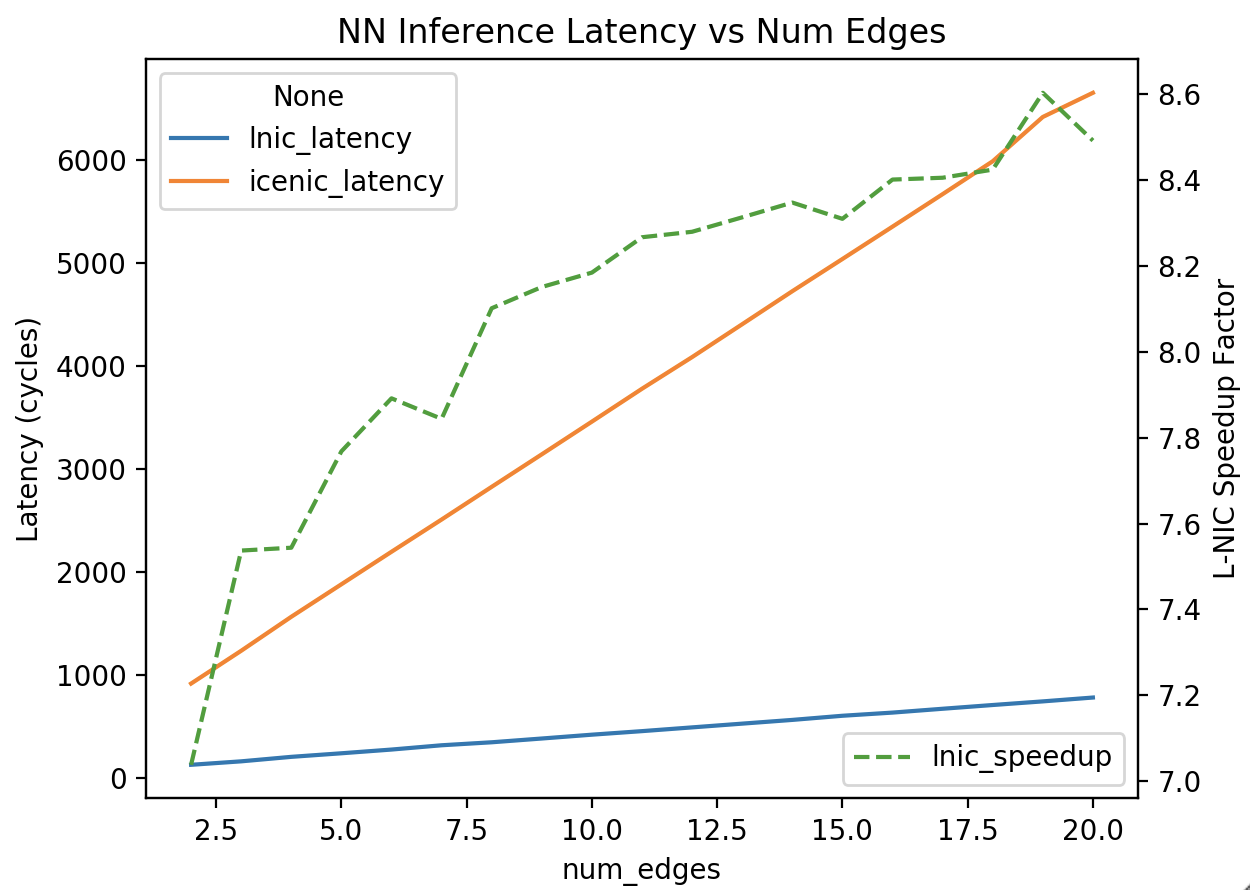
\includegraphics[width=\linewidth]{./figures/nn-inference-latency}
%  \caption{\name{} vs Traditional neural network node latency for various number of incoming edges.}
%  \label{fig:nn-latency}
%\end{figure}

\paragraph{Othello Map/Reduce.} We re-implemented the Othello application (used as a benchmark in~\cite{lnic}), comparing its performance on the \name{} with a Traditional design.
An Othello board can be represented by just two 64-bit unsigned integers, hence the working set fits in the L1 cache. The set of possible next moves can be calculated in less than one microsecond, as demonstrated in \cite{lnic}.

We measured the latency of the ``map'' and ``reduce'' operations as a function of the {\em fanout}, which is the number of possible next moves given an initial board state.
Because of the very short execution latency and the \name{}'s superior TX/RX throughput, the \name{} reduces the time for both operations by a factor of 4--6$\times$ (Figure~\ref{fig:latency}d,e).

%\begin{figure}
%  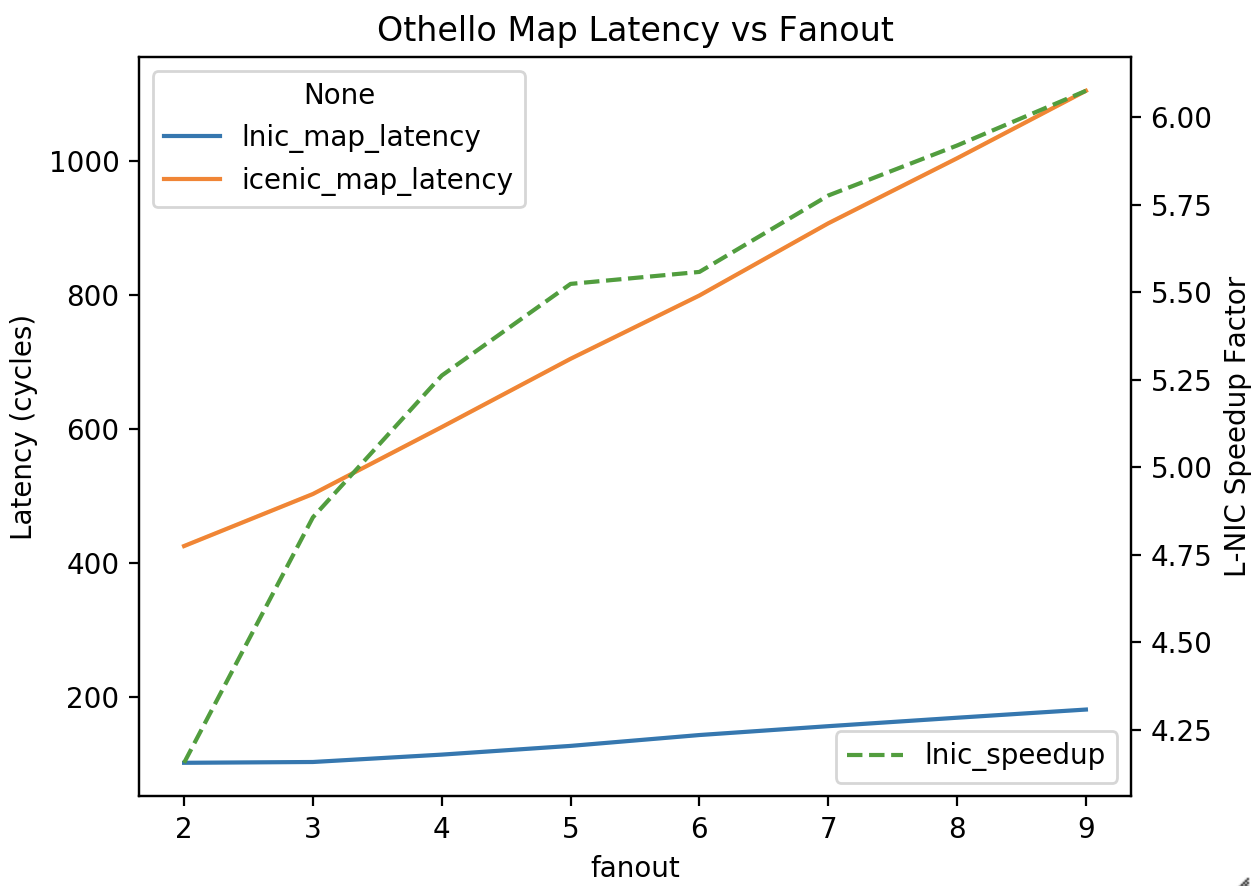
\includegraphics[width=\linewidth]{./figures/othello-map-latency}
%  \caption{\name{} vs Traditional Othello map latency for various degrees of fanout.}
%  \label{fig:othello-map-latency}
%\end{figure}
%
%\begin{figure}
%  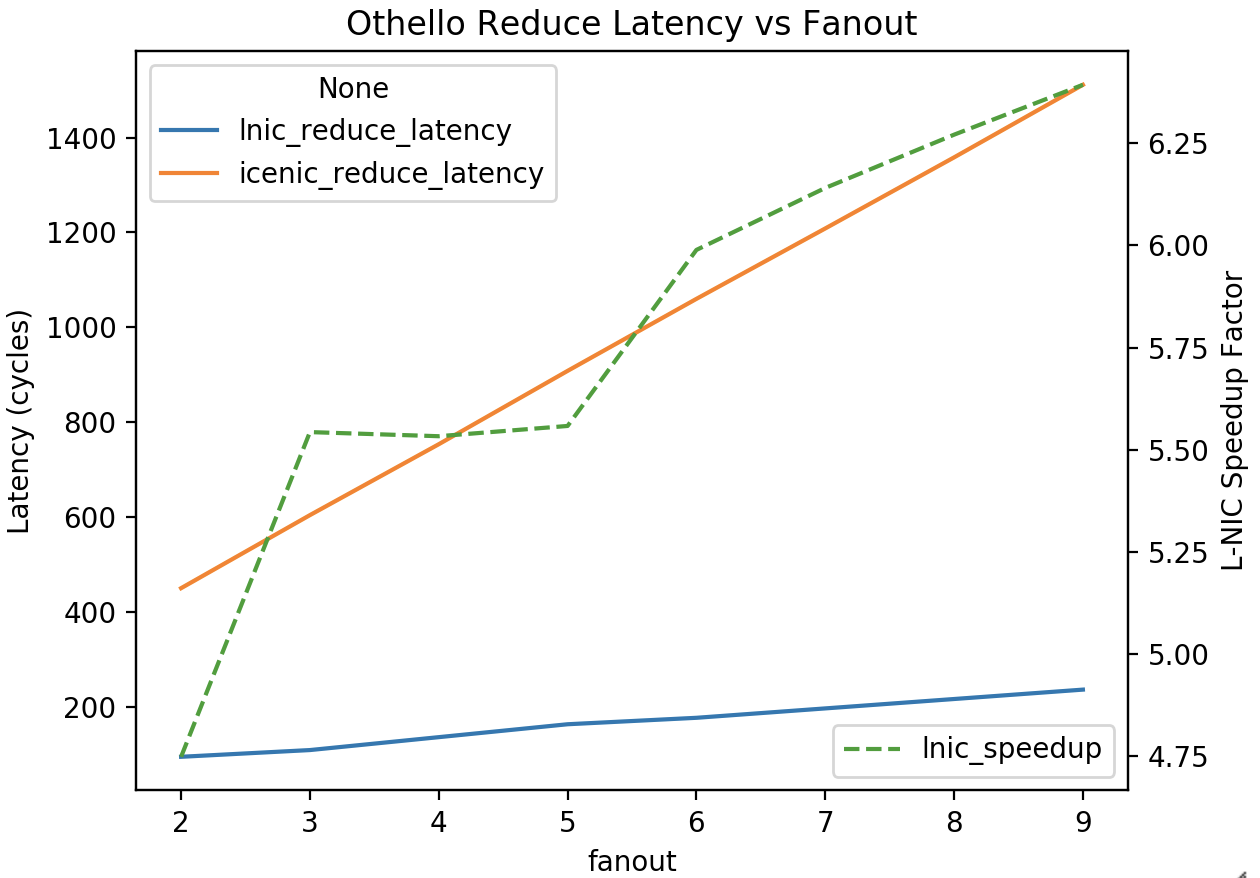
\includegraphics[width=\linewidth]{./figures/othello-reduce-latency}
%  \caption{\name{} vs Traditional Othello reduce latency for various degrees of fanout.}
%  \label{fig:othello-reduce-latency}
%\end{figure}

\paragraph{N-body Simulation.} Nanoservices can efficiently implement and execute N-body simulations.
This scientific computing application is typically run on HPC clusters. 
Astronomers use N-body simulations to model the gravitational interaction of celestial bodies.
These simulations are computationally heavy, with most time spent computing the gravitational force each body exerts on every other body.
A popular data structure for N-body simulations is a quad-tree, as described in the Barnes-Hut algorithm~\cite{barnes-hut}. 
This algorithm reduces the computational complexity required for the gravity computation step from $O(N^2)$ to $O(N \log N)$.

A na\"ive nanoservices implementation of the Barnes-Hut algorithm would simply implement each node of the quad-tree as a separate nanotask and pass messages between nanotasks to compute gravitational forces, as shown in Figure~\ref{fig:barnes-hut}. 
Leaf nodes represent bodies being simulated and internal nodes represent regions of space. 
To compute the force exerted on body F, node F will send a message intended to traverse the quadtree, starting at the root. 
If the center of mass of the receiving node is sufficiently far away, the current node will compute the force that it exerts on body F and return the result in a response message. 
Otherwise, the node will forward the request to all of its children, which recursively implement the same procedure.

In the Barnes-Hut algorithm, the state per node would be L1 cache resident, consisting primarily of the node's position and mass.
A node computes the force it exerts on the body identified by the arriving message, using the equation
 $F_G = G\frac{m_1 \cdot m_2}{r^2} $
where, $G$ is the gravitational constant, $m_1$ and $m_2$ are the masses of the two bodies, and $r$ is the distance between them.
Thus, the computation only requires a few floating point operations and the response time for each message is easily $<1\mu$s. 
This is a radical departure from how the Barnes-Hut algorithm is implemented today in Changa~\cite{changa}, in which the quad-tree is stored as a large in-memory data structure distributed across many machines.

We implemented and measured a single node of an N-body physical simulation. Latency is measured from when the first byte of the first request message enters the NIC to when the last byte of the last response message leaves the NIC.
As shown in Figure~\ref{fig:latency}f, the \name{} reduces latency by $2.5\times$ compared to a Traditional design. 
Section~\ref{ssec:large-eval} describes a large-scale evaluation of the N-body physical simulation across multiple nodes. 

\begin{figure}
 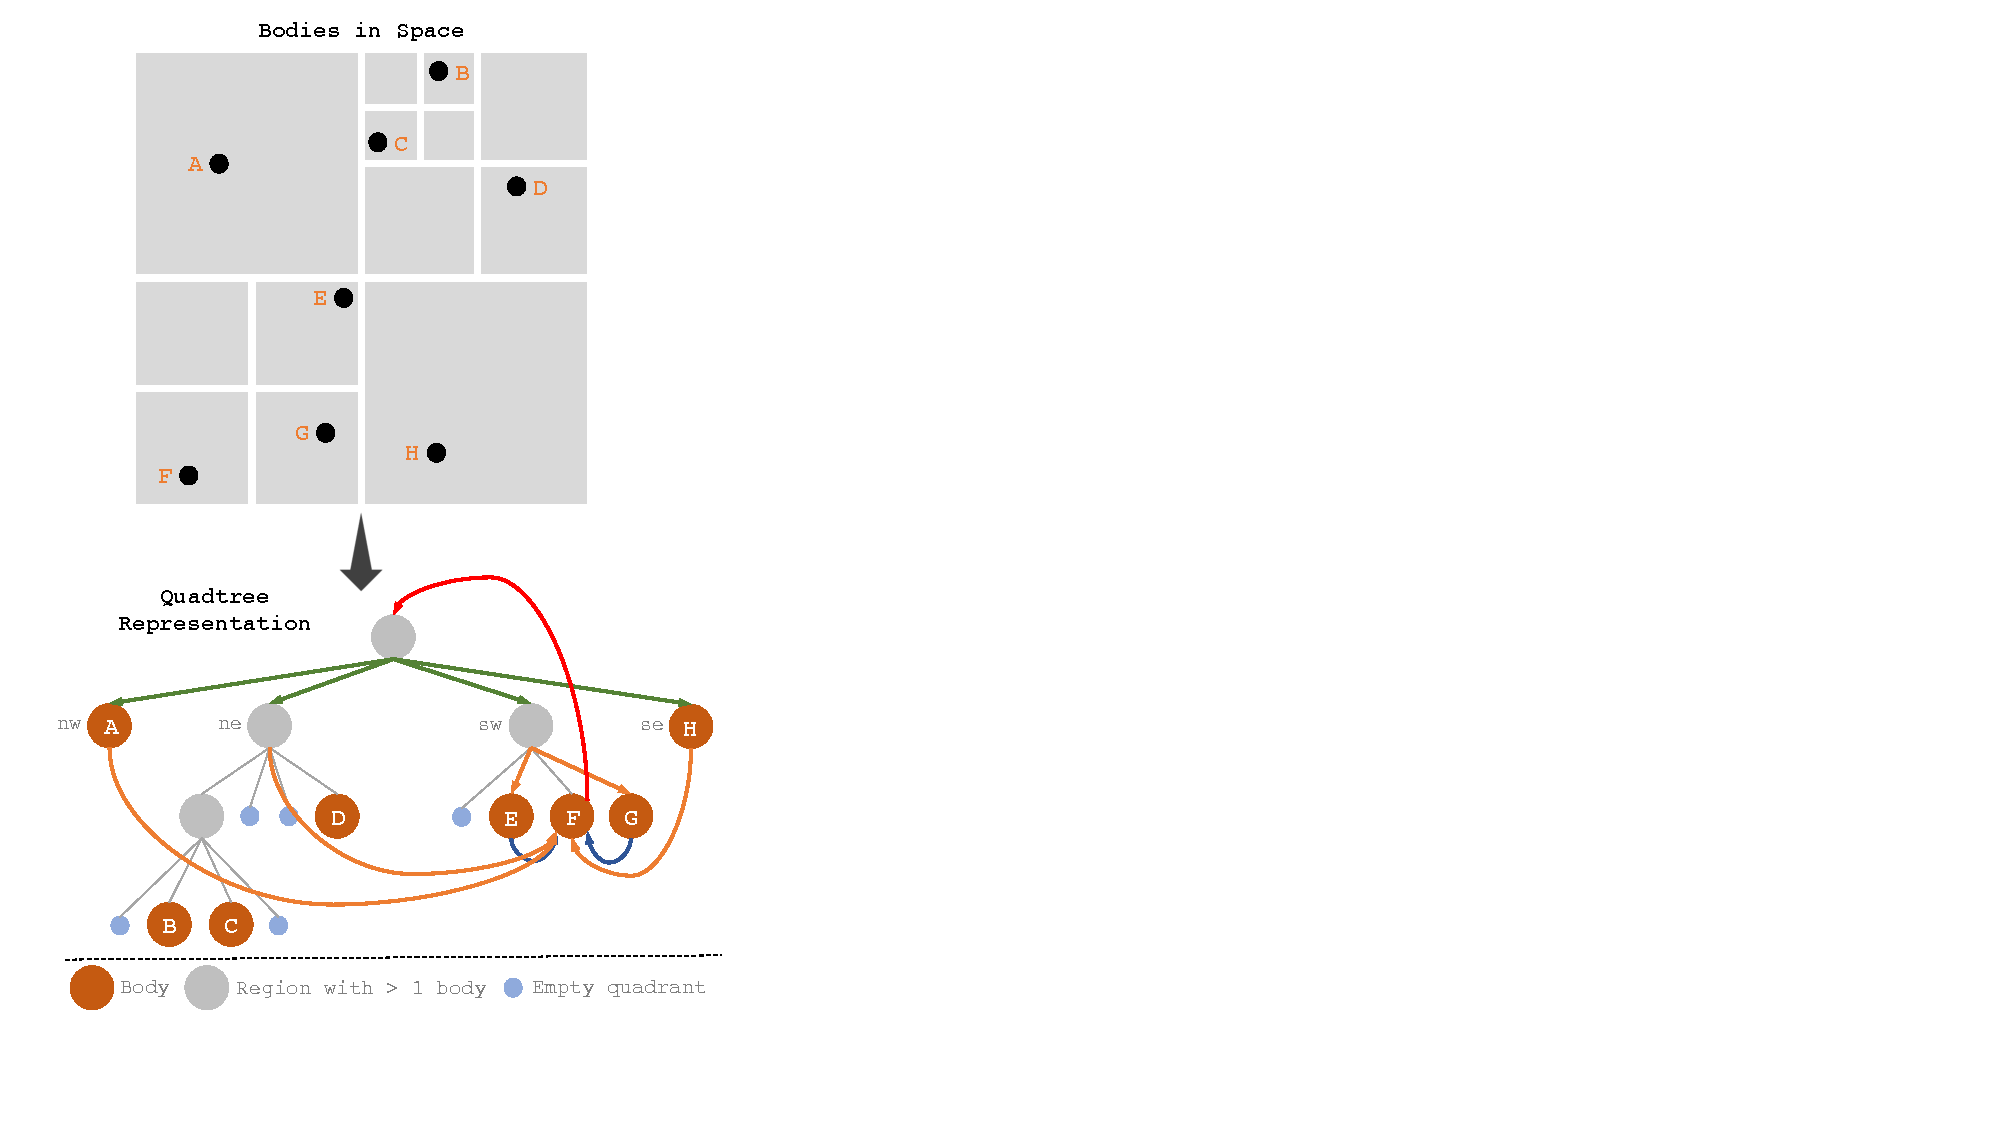
\includegraphics[width=0.9\linewidth]{./figures/barneshut-algo}
 \caption{An example message-passing pattern to compute the gravitational forces exerted on body F using a simple nanoservices implementation of the Barnes-Hut algorithm~\cite{barnes-hut}.}
 \label{fig:barnes-hut}
\end{figure}

\subsection{Thread Scheduling Benchmarks}
We compare two thread scheduling policies. The first is our NIC-driven hardware thread scheduling policy described in Section~\ref{ssec:thread-scheduler}, in which the NIC decides which thread to run next and tells the CPU via the CSR registers. The second represents a more traditional Linux-style, timer-driven thread scheduler, in which timer interrupts are configured to fire periodically to decide which thread to run next and NIC hardware interrupts are disabled.
In both cases, when an interrupt fires, the processor traps into the nanokernel, which then swaps to the highest priority context with messages to process.
The key difference is that in the timer-driven approach, context switches only happen on periodic time boundaries, hence we can expect them to have longer latency (both average and tail).

To compare the two scheduling policies we pin one high-priority context and one low-priority context on the core, then send in a stream of randomly interleaved high- and low-priority requests (separated by an interpacket gap of \SI{500}{ns}).
Each application services the request for \SI{500}{ns} (1500 instructions) before sending back a response. 

Figure~\ref{fig:scheduling-latency} compares the two scheduling policies by measuring the distribution of response times for high-priority messages.
Our hardware NIC-driven scheduling policy reduces the tail response latency by a factor of $5.5\times$ and the standard deviation of the response times by almost $20\times$.
This result should not be surprising--the NIC-driven scheduling policy is able to immediately evict the low-priority thread once a high-priority message arrives, whereas the timer-driven policy must wait for a timer interrupt.
The NIC-driven scheduling policy also accelerates the low-priority application because the timer-driven policy causes many traps into the nanokernel for no particular reasons, degrading its throughput. Our evaluation demonstrates the huge potential benefit of allowing the NIC hardware to drive the context-switch logic.

\begin{figure}
  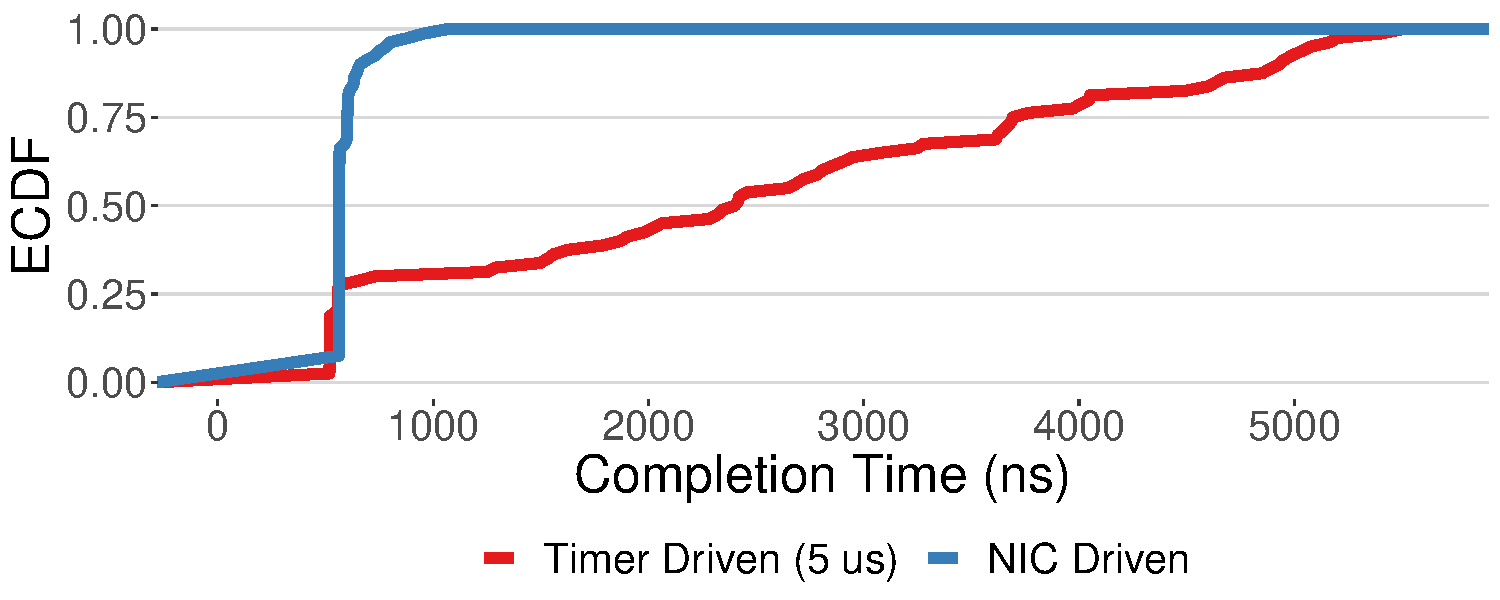
\includegraphics[width=\linewidth]{./figures/scheduling-comptimes}
  \caption{Latency reduction as a result of NIC-driven thread scheduling relative to timer-driven thread scheduling.}
  \label{fig:scheduling-latency}
\end{figure}

%\begin{figure}
%  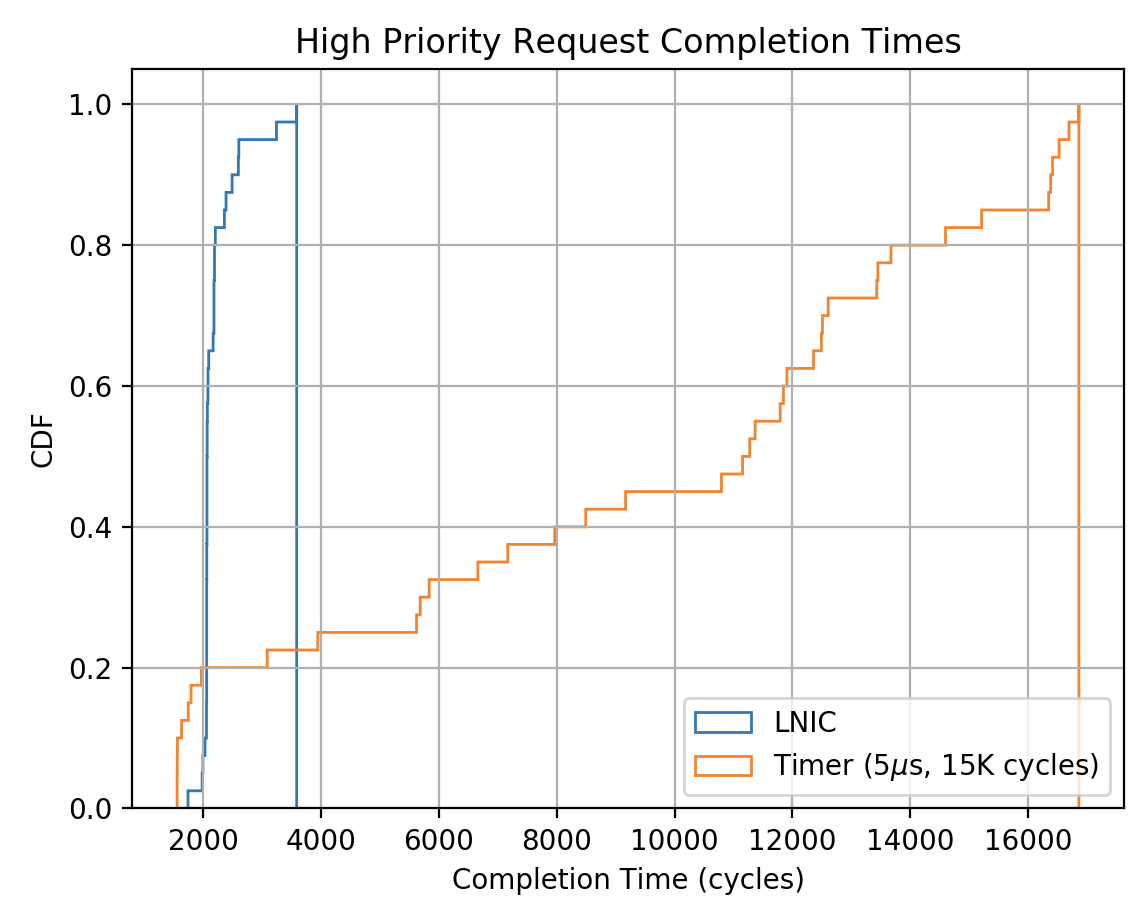
\includegraphics[width=\linewidth]{./figures/scheduling-tail-latency}
%  \caption{Latency reduction as a result of NIC-driven thread scheduling relative to timer-driven thread scheduling.}
%  \label{fig:scheduling-latency}
%\end{figure}

\subsection{Large-Scale N-Body Simulation}
\label{ssec:large-eval}
We demonstrate the huge performance gains of a large-scale nanoservice deployment using N-body simulation and the na\"ive nanoservice implementation, described in~\S\ref{ssec:bare-metal-evals}.
In this approach, the root node of the quad-tree becomes the bottleneck, because it must process one message from each body being simulated, and the root node dictates the total runtime of the gravity computation step.
We compare the performance of our na\"ive nanoservice application with the performance obtained when using ChanGa~\cite{changa}, a popular N-body gravitational simulator.

Table~\ref{tab:nbody-changa} compares the average gravity computation time for 80K bodies using both the ChanGa simulator (with recommended parameter settings) and the na\"ive nanoservices implementation.
We obtain the expected nanoservice performance by extrapolating the performance of the \name{} bare-metal N-body node, evaluated in \S\ref{ssec:bare-metal-evals}, to 80K messages, mimicking the processing required by the root node of the quad-tree.
Even our simple, na\"ive nanoservice implementation will reduce the total gravity computation time by four orders of magnitude. We can drive it down further by replicating certain nodes of the quad-tree.
Although ChanGa is widely used, we can significantly outperform it because, unlike nanoservices, it uses very coarse-grained parallelism. Note that our evaluation assumes the transport protocol is able to handle an 80K-to-1 incast without ever overflowing or underflowing the receiver buffer.
This type of massive incast is not special to this one application, but we expect that this will be common across many nanoservice applications.
Designing or adopting transport protocols to deal with this degree of incast may be challenging and is a subject of future research.

\begin{table}
\begin{center}
\begin{tabular}{c|c}
                      & \textbf{Avg. Gravity Computation Time} \\ \toprule
\textbf{Nanoservices} & 4 ms                                   \\
\textbf{ChanGa}       & 30,000 ms                                 \\
\end{tabular}
\vspace{5pt}
\caption{Comparing the average gravity computation time in an N-body simulation of 80K bodies using a theoretical nanoservices deployment and a real implementation using ChanGa~\cite{changa}.}
\label{tab:nbody-changa}
\end{center}
\end{table}